\chapter{Thực nghiệm}

Chương này trình bày kết quả thực nghiệm của khóa luận theo ba câu hỏi nghiên cứu đã đặt ra ở Chương 1. RQ1 xét giá trị của thông tin sự kiện đối với quyết định hành động và tỷ lệ hoàn thành tác vụ. RQ2 xét hành vi của cơ chế kiểm định bằng chứng và truy vấn theo sự kiện khi lịch sử chưa đầy đủ. RQ3 xét khả năng duy trì kỹ năng cơ sở sau thích ứng và khả năng áp dụng công thức thích ứng cho một kiến trúc VLA khác. Tương ứng với đóng góp thứ ba, các thực nghiệm được tổ chức theo ba tầng: tầng vòng kín có đối chứng trên LIBERO-Mem, tầng quyết định cục bộ với can thiệp lời nhắc tại đúng một truy vấn, và tầng duy trì kỹ năng trên LIBERO-10 với hai mô hình nền. Kiểm tra truy vấn theo sự kiện đồng thời là phép kiểm tra vận hành của kiến trúc bộ nhớ và cơ chế điều phối được đề xuất trong đóng góp thứ hai.

Bảng~\ref{tab:experiment-rq-map} tóm tắt quan hệ giữa các thực nghiệm, câu hỏi nghiên cứu, đóng góp và quy mô mẫu. Quy mô mẫu được nêu kèm từng kết quả để xác định đúng mức độ chắc chắn của mỗi nhận định. Mọi cohort trong chương đều chạy theo giao thức riêng của khóa luận và không so sánh trực tiếp với điểm số công bố chính thức của LIBERO hay LIBERO-Mem.

\begingroup\small\setlength{\tabcolsep}{4pt}\renewcommand{\arraystretch}{1.15}
\begin{longtable}{>{\raggedright\arraybackslash}p{\dimexpr 0.24\textwidth-2\tabcolsep\relax}>{\raggedright\arraybackslash}p{\dimexpr 0.10\textwidth-2\tabcolsep\relax}>{\raggedright\arraybackslash}p{\dimexpr 0.12\textwidth-2\tabcolsep\relax}>{\raggedright\arraybackslash}p{\dimexpr 0.24\textwidth-2\tabcolsep\relax}>{\raggedright\arraybackslash}p{\dimexpr 0.30\textwidth-2\tabcolsep\relax}}
\caption{Ánh xạ giữa thực nghiệm, câu hỏi nghiên cứu và đóng góp}\label{tab:experiment-rq-map}\\
\toprule
\textbf{Thực nghiệm} & \textbf{RQ} & \textbf{Đóng góp} & \textbf{Quy mô} & \textbf{Vai trò bằng chứng} \\
\midrule\endfirsthead
\toprule
\textbf{Thực nghiệm} & \textbf{RQ} & \textbf{Đóng góp} & \textbf{Quy mô} & \textbf{Vai trò bằng chứng} \\
\midrule\endhead
\bottomrule\endfoot
Đối sánh vòng kín, F0 và F1 trên LIBERO-Mem & RQ1 & 3 & 40 cặp, 80 lượt & Đối sánh vòng kín chính về tác động của bộ nhớ \\
Kiểm tra truy vấn theo sự kiện trên nhóm phát triển, shadow và event & RQ2 & 2, 3 & 24 cặp, 48 lượt & Kiểm tra đường kích hoạt truy vấn theo bằng chứng \\
Kiểm tra truy vấn theo sự kiện trên nhóm hiệu chuẩn sau override & RQ2 & 2, 3 & 16 cặp, 32 lượt & Chẩn đoán phát triển trên nhóm trạng thái thứ hai \\
Bỏ bộ nhớ tại một truy vấn & RQ1 & 3 & 2 ca, mỗi ca 2 nhánh & Độ nhạy cục bộ của rollout đối với lời nhắc \\
Duy trì hiệu năng SmolVLA, B0 và F1-off & RQ3 & 3 & 50 cặp, 100 lượt & Duy trì kỹ năng trên mô hình nền chính \\
Duy trì hiệu năng X-VLA, B0, F0 và F1-off & RQ3 & 3 & 50 bộ ba, 150 lượt & Duy trì kỹ năng trên mô hình nền thứ hai \\
\end{longtable}
\endgroup

\section{Thiết lập thực nghiệm và chỉ số đánh giá}

\subsection{Các điều kiện đối chứng}

Để đánh giá một cách khoa học và bóc tách rõ vai trò của từng thành phần, nghiên cứu thiết lập bốn điều kiện đối chứng có kiểm soát chặt chẽ:

\begin{enumerate}
    \item \textbf{Mô hình cơ sở gốc (B0):} Sử dụng checkpoint tiền huấn luyện chính thức của SmolVLA mà không qua bất kỳ bước tinh chỉnh nào, chỉ tiếp nhận chỉ dẫn ngôn ngữ ban đầu $\ell$. Điều kiện này đóng vai trò là mốc tham chiếu hiệu năng zero-shot của mô hình nền tảng.
    \item \textbf{Đối chứng thích ứng không bộ nhớ (F0):} Mô hình SmolVLA được tinh chỉnh LoRA trên Action Expert với cùng bộ dữ liệu và cùng ngân sách 5.000 bước tối ưu, nhưng chỉ nhận chỉ dẫn ngôn ngữ gốc $\ell$ mà không có thông tin bộ nhớ. Điều kiện này là mốc đối chứng then chốt để đo lường riêng biệt tác động của việc bổ sung ngữ cảnh bộ nhớ.
    \item \textbf{Chính sách có bộ nhớ đề xuất (F1):} Mô hình được huấn luyện và suy luận với đầy đủ thông tin bộ nhớ sự kiện có bằng chứng được chiếu thành văn bản $C_q$. Cả F0 và F1 đều chia sẻ chung checkpoint nền, tập quỹ đạo huấn luyện, cấu hình LoRA và siêu tham số tối ưu hóa.
    \item \textbf{Kiểm định độ nhạy cắt bộ nhớ (F1-off):} Sử dụng nguyên vẹn trọng số đã học của F1 nhưng chủ động cắt bỏ phần văn bản bộ nhớ trong quá trình suy luận vòng kín, chỉ cung cấp chỉ dẫn gốc. Đối chứng này nhằm kiểm định xem mô hình có thực sự học cách điều kiện hóa hành vi dựa trên tín hiệu bộ nhớ hay không.
\end{enumerate}

Bảng~\ref{tab:experimental-conditions} tổng hợp cấu hình của bốn điều kiện thực nghiệm.

\begingroup\small\setlength{\tabcolsep}{4pt}\renewcommand{\arraystretch}{1.15}
\begin{longtable}{>{\raggedright\arraybackslash}p{\dimexpr 0.18\textwidth-2\tabcolsep\relax}>{\raggedright\arraybackslash}p{\dimexpr 0.26\textwidth-2\tabcolsep\relax}>{\raggedright\arraybackslash}p{\dimexpr 0.26\textwidth-2\tabcolsep\relax}>{\raggedright\arraybackslash}p{\dimexpr 0.30\textwidth-2\tabcolsep\relax}}
\caption{Các điều kiện thực nghiệm đối chứng}\label{tab:experimental-conditions}\\
\toprule
\textbf{Điều kiện} & \textbf{Trọng số mô hình} & \textbf{Ngữ cảnh văn bản} & \textbf{Mục đích đánh giá} \\
\midrule\endfirsthead
\toprule
\textbf{Điều kiện} & \textbf{Trọng số mô hình} & \textbf{Ngữ cảnh văn bản} & \textbf{Mục đích đánh giá} \\
\midrule\endhead
\bottomrule\endfoot
B0 & Checkpoint gốc & Chỉ dẫn gốc & Mốc tham chiếu nền tảng trước thích ứng \\
F0 & Adapter LoRA đối chứng & Chỉ dẫn gốc & Đo lường tác động của thích ứng không bộ nhớ \\
F1 & Adapter LoRA có bộ nhớ & Chỉ dẫn và sự kiện & Đánh giá hiệu quả của phương pháp đề xuất \\
F1-off & Trọng số của F1 & Chỉ dẫn gốc & Kiểm tra độ nhạy và phụ thuộc vào bộ nhớ \\
\end{longtable}
\endgroup

Khi có dữ kiện hợp lệ trong ngân sách token, F1 nối các câu dữ kiện sau chỉ dẫn gốc bằng tiền tố \texttt{Memory:}. Hình~\ref{fig:prompt-example} trích hai lời nhắc từ cùng lượt T1: chỉ dẫn gốc tại bước 0 và lời nhắc tại bước 312, khi bộ nhớ ghi nhận một lần bát trở về. Cụm \texttt{History incomplete.} cho biết lịch sử quan sát vẫn chưa đầy đủ.

\begin{figure}[htbp]
\centering
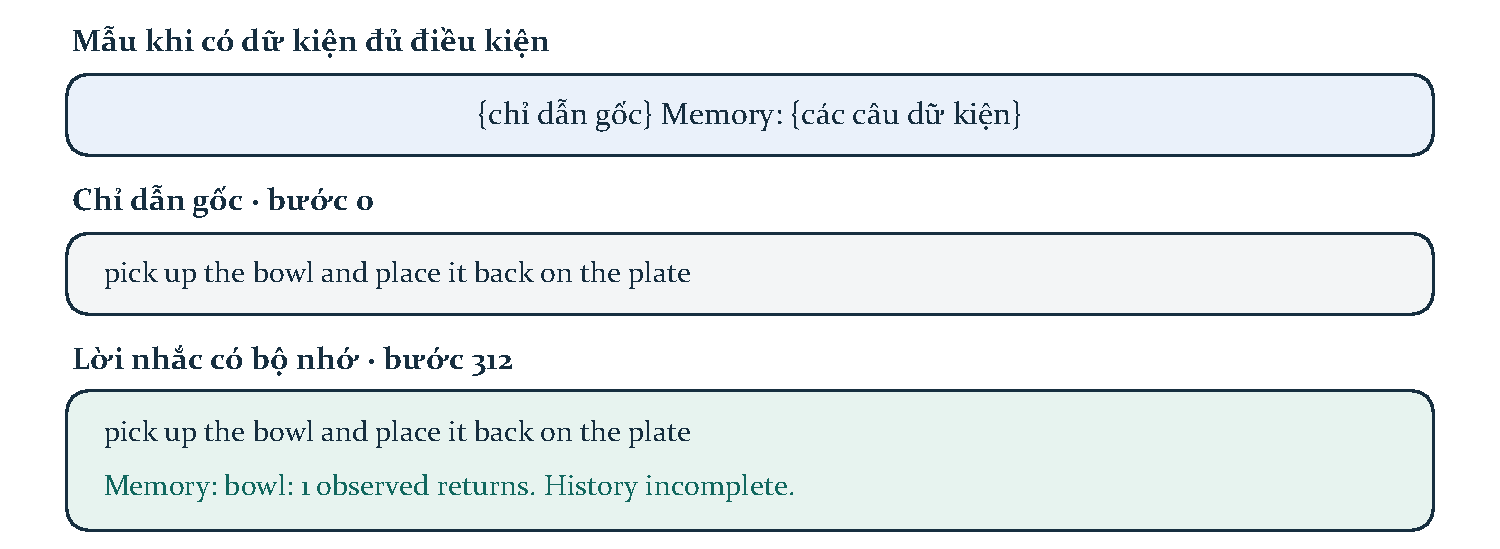
\includegraphics[width=.96\linewidth]{../figures/loi-nhac-bo-nho.pdf}
\caption{Mẫu lời nhắc bộ nhớ và ví dụ từ nhật ký T1}
\label{fig:prompt-example}
\end{figure}

\subsection{Giao thức mô phỏng và chỉ số đánh giá}

Các thử nghiệm vòng kín được thực hiện trên môi trường mô phỏng cánh tay robot Franka Emika Panda với bộ điều khiển không gian tác vụ Operational Space Controller OSC\_POSE vận hành ở tần số 20 Hz. Hệ thống cảm biến cung cấp hai luồng ảnh RGB kích thước $256 \times 256$ (camera góc nhìn thứ ba và camera gắn cổ tay) cùng vector trạng thái khớp robot.

Mỗi lượt thực thi bắt đầu bằng 20 bước làm nóng để ổn định tiếp xúc vật lý. Chính sách VLA sinh đoạn hành động gồm $H = 50$ lệnh chuyển động và thực thi $K = 10$ hành động trước khi truy vấn lại. Mỗi lượt chạy có giới hạn tối đa 1.000 bước hành động. Một lượt bị dừng sớm nếu bộ chấm phát hiện hành vi vượt quá số chu kỳ yêu cầu.

Để định lượng hiệu năng một cách toàn diện, nghiên cứu sử dụng ba chỉ số đánh giá:
\begin{enumerate}
    \item \textbf{Chỉ báo thành công toàn phần ($S_i$):}
    \begin{equation}
    S_i = \mathbf{1}[K_i = K_i^\star \land P_i \land \neg O_i].
    \end{equation}
    Trong đó $K_i$ là số mốc chu kỳ bộ chấm xác nhận, $K_i^\star$ là số mốc yêu cầu của tác vụ, $P_i$ là vị từ kiểm tra trạng thái đích tại thời điểm kết thúc, và $O_i$ là cờ báo vi phạm vượt số chu kỳ.
    \item \textbf{Tỷ lệ hoàn thành mốc thành phần ($\mathrm{SCR}_i$):} Đo lường tiến độ từng phần của robot:
    \begin{equation}
    \mathrm{SCR}_i = \frac{K_i}{K_i^\star}.
    \end{equation}
    \item \textbf{Tỷ lệ thành công thực nghiệm ($\widehat{\mathrm{SR}}$):} Trung bình tỷ lệ thành công trên tập $M$ lượt đánh giá:
    \begin{equation}
    \widehat{\mathrm{SR}} = \frac{1}{M}\sum_{i=1}^{M} S_i.
    \end{equation}
\end{enumerate}

\subsection{Mô hình nền thứ hai X-VLA}
\label{sec:xvla-setup}

Để trả lời phần mở rộng kiến trúc của RQ3, khóa luận lặp lại công thức thích ứng F0/F1 trên X-VLA \cite{xvla2025}. X-VLA dùng bộ mã hóa thị giác--ngôn ngữ Florence-2, soft prompt theo từng embodiment và đầu hành động flow matching. Điều kiện B0 của X-VLA là checkpoint X-VLA-Libero do nhóm tác giả công bố (revision \texttt{129e7146}). Khác với SmolVLA, X-VLA dự đoán tư thế tuyệt đối của đầu gắp, gồm vị trí, biểu diễn quay 6D và xác suất đóng gắp. Mỗi đoạn hành động gồm 30 bước và được thực thi trọn vẹn trước lần truy vấn kế tiếp, với 10 bước tích phân flow và tần số điều khiển 20 Hz. Vì vậy, lệnh delta trong dữ liệu huấn luyện V2 được chuyển sang tư thế tuyệt đối bằng phép tính giải tích. Tập huấn luyện dùng cùng khóa phân chia với SmolVLA, gồm 109.945 khung cơ sở và 42.857 khung LIBERO-Mem.

Hai adapter X-VLA F0 và F1 được huấn luyện 5.000 bước với cùng công thức. Phần tham số được cập nhật gồm các ma trận LoRA và một số mô-đun được huấn luyện đầy đủ, tổng cộng khoảng 11,87 triệu tham số. Batch hiệu dụng là 32, tốc độ học $5\times10^{-5}$ với 250 bước khởi động và lịch cosine giảm về 0,1 lần giá trị ban đầu, seed 42. Khác biệt duy nhất giữa hai adapter là ngữ cảnh văn bản: F0 nhận chỉ dẫn gốc, còn F1 nhận lời nhắc bộ nhớ do bộ ghi quan hệ RGB phiên bản V1 sinh ra. Hai adapter xuất ra có mã băm khác nhau. Các lượt X-VLA trên LIBERO-Mem chưa đủ cohort tại thời điểm viết, nên chương này chỉ báo cáo X-VLA trong phép đánh giá duy trì hiệu năng sau tinh chỉnh, với bộ nhớ tắt ở cả ba điều kiện.

\section{Đối sánh vòng kín trên LIBERO-Mem}

% claim-id: v2-data
% claim-id: writer-checkpoint-comparison
Thực nghiệm đối sánh vòng kín so sánh đối đầu giữa hai adapter F0 và F1 trên cùng 20 nhóm trạng thái kiểm tra Unseen (\texttt{demo\_101}--\texttt{demo\_120}) của hai tác vụ T1 (yêu cầu một chu kỳ nhấc và đặt lại bát) và T3 (yêu cầu ba chu kỳ). Hai cấu hình được ghép cặp chặt chẽ theo từng trạng thái khởi tạo và hạt giống ngẫu nhiên seed 42, tạo thành 40 cặp đối đầu với tổng cộng 80 lượt chạy vòng kín độc lập.

Các bản ghi thực nghiệm đối sánh vòng kín vận hành ở chế độ suy luận định kỳ tiêu chuẩn ($K = 10$ hành động giữa hai lần truy vấn chính sách), tập trung đánh giá tác động của việc điều kiện hóa ngữ cảnh văn bản lên phân phối hành động của VLA.

\begin{table}[htbp]
\centering\small
\caption{Kết quả đối sánh vòng kín đối sánh vòng kín trên tác vụ T1 và T3}
\label{tab:e2-unseen-results}
\begin{tabular}{lrrrr}
\toprule
& \multicolumn{2}{c}{\textbf{Thành công toàn phần}} & \multicolumn{2}{c}{\textbf{Chưa đạt mốc nào}} \\
\cmidrule(lr){2-3}\cmidrule(lr){4-5}
\textbf{Tác vụ} & \textbf{F0} & \textbf{F1} & \textbf{F0} & \textbf{F1} \\
\midrule
T1 & 3/20 & 0/20 & 15/20 & 19/20 \\
T3 & 1/20 & 0/20 & 15/20 & 18/20 \\
\textbf{Tổng} & \textbf{4/40} & \textbf{0/40} & \textbf{30/40} & \textbf{37/40} \\
\bottomrule
\end{tabular}
\end{table}

Trên 40 cặp đối sánh vòng kín, F1 đạt 0/40 thành công so với 4/40 của F0; chênh lệch SR là $-10$ điểm phần trăm, với khoảng bootstrap 95\% theo 20 cụm trạng thái từ $-20$ đến $-2{,}5$ điểm. F1 không đạt mốc nào ở 37/40 lượt, so với 30/40 của F0. Các log cho thấy khác biệt về tiến độ và thời gian chạy, nhưng không xác định nguyên nhân lỗi. Trong stack đồng bộ đã dùng, trung vị wall time là khoảng 213 giây với F0 và 1.066 giây với F1.

Đối chứng raw B0 bổ sung chạy trên cùng 40 hash trạng thái và seed 42 đạt 0/40 thành công, mean SCR $0{,}0167$, không overshoot; T1 đạt 0/20 và T3 đạt 0/20, trong đó một lượt T3 hoàn thành 2/3 mốc. Đây chỉ là đối chiếu mô tả: 115/134 source hash trùng đối sánh vòng kín và policy runtime khác nhau (B0 WSL Torch 2.11/CUDA 12.8; đối sánh vòng kín Windows Torch 2.6/CUDA 12.4). Vì vậy không dùng B0--đối sánh vòng kín để quy hiệu quả cho fine-tuning hoặc memory, và không gộp thành điểm LIBERO chính thức.

% claim-id: t3-success-video
Hình~\ref{fig:t3-pilot-success} minh họa lượt T3 thành công của pilot lịch sử, test state 2. Ba cột đầu ứng với 1/3, 2/3 và 3/3 mốc tích lũy; cột cuối là lúc kết thúc. Hàng trên là camera ngoài, hàng dưới là camera cổ tay. Bộ ghi xác nhận hai lượt trở về và đánh dấu lịch sử chưa đầy đủ. Lượt này dùng checkpoint lịch sử và nằm ngoài cohort đối sánh vòng kín.

\begin{figure}[htbp]
\centering
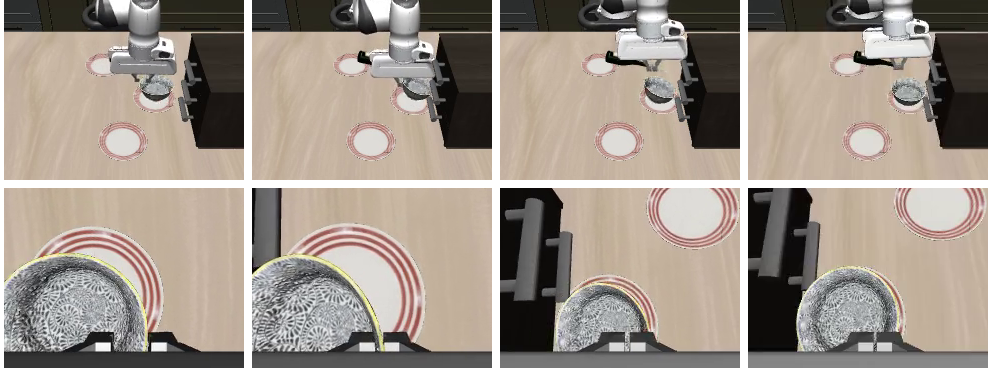
\includegraphics[width=.96\linewidth]{../figures/t3-ba-moc.png}\par
{\small\makebox[.24\linewidth]{Bước 190}%
\makebox[.24\linewidth]{Bước 626}%
\makebox[.24\linewidth]{Bước 863}%
\makebox[.24\linewidth]{Bước 1.000}\par}
\caption{Ba mốc thao tác của lượt T3 thành công trong pilot}
\label{fig:t3-pilot-success}
\end{figure}

\section{Duyệt theo bằng chứng trong vòng kín}
\label{sec:d2-evidence}

% claim-id: open-policy-gate
Để kiểm tra trực tiếp cơ chế điều phối, thực nghiệm ghép cặp hai chế độ trên cùng 12 trạng thái seen của T1 và T3, cùng checkpoint F1, seed 42 và query horizon cơ sở 10 hành động (24 episode mỗi chế độ). Arm shadow chỉ ghi quyết định giám sát; arm event có thể phát truy vấn sớm khi memory đổi ngữ nghĩa và có evidence. Hash trạng thái khởi tạo khớp ở cả 24 cặp. Đây là cohort phát triển V2 tùy biến, không phải điểm LIBERO chính thức.

\begin{table}[htbp]
\centering\small
\caption{Kết quả kiểm tra truy vấn theo sự kiện trên cohort phát triển T1/T3 (24 episode mỗi arm)}
\label{tab:d2-decision-results}
\setlength{\tabcolsep}{4pt}
\begin{tabular}{lrrrrrr}
\toprule
\textbf{Arm} & \textbf{Thành công} & \shortstack{\textbf{SCR}\\\textbf{trung bình}} & \shortstack{\textbf{Lần gọi VLA}\\\textbf{/lượt}} & \shortstack{\textbf{Lượt có}\\\textbf{gọi sớm}} & \shortstack{\textbf{Có mã}\\\textbf{evidence}} & \shortstack{\textbf{Thêm mã}\\\textbf{mới}} \\
\midrule
Shadow-projected & 1/24 & 0,111 & 97,17 & 0/24 & -- & -- \\
Event-projected & 1/24 & 0,167 & 99,88 & 22/24 & 56/56 & 41/56 \\
\bottomrule
\end{tabular}
\end{table}

% claim-id: d2-requery-evidence-freshness
Event mode đã kích hoạt requery trong closed loop: cả 56 lần gọi sớm đều ghi mã evidence, nhưng chỉ 41 lần thêm ID mới. 15 lần còn lại chỉ gắn ``History incomplete'' vào fact bát và giữ 9 ID từ quan sát bước 0--2; tuổi evidence của chúng có median 73 hành động (32--758). Không có ngưỡng tuổi định trước, nên đây là mô tả độ mới trong log, không phải đánh giá đúng sai. Hai episode không phát requery. Hai chế độ đều đạt 1/24 success, nhưng ở hai state khác nhau; chênh lệch SCR trung bình là $+0{,}056$ với khoảng bootstrap theo nhóm state 95\% từ $-0{,}125$ đến $0{,}250$. Kết quả development xác nhận đường kích hoạt, chưa chứng minh lợi ích hiệu năng. Lượt T1 state 7 của event đạt mốc ở bước 409 và terminal success ở bước 1.000; shadow thành công ở state 5.

\begin{figure}[htbp]
\centering
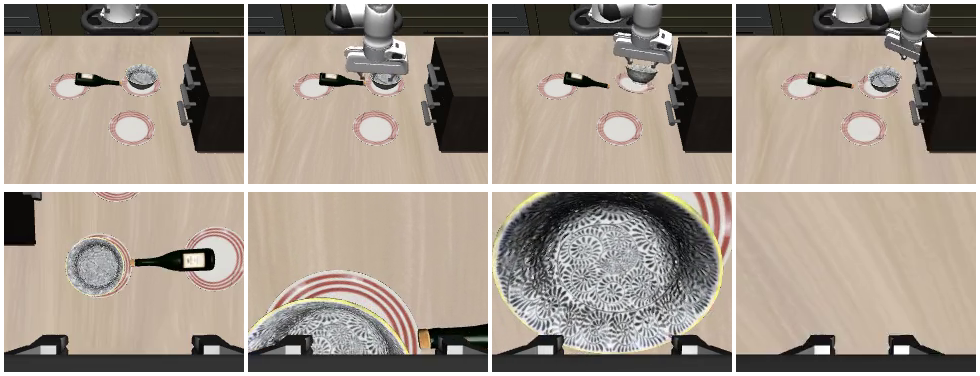
\includegraphics[width=\linewidth]{../figures/t1-truy-van-som.png}\par
{\small\makebox[.25\linewidth]{Bước 0}%
\makebox[.25\linewidth]{Bước 142}%
\makebox[.25\linewidth]{Bước 409}%
\makebox[.25\linewidth]{Bước 1.000}\par}
\caption{Lượt T1 thành công có truy vấn sớm}
\label{fig:libero-mem-d2-t1-success}
\end{figure}

Trong Hình~\ref{fig:libero-mem-d2-t1-success}, hàng trên là camera ngoài, hàng dưới là camera cổ tay. Hình~\ref{fig:t1-grasp-detail} phóng to vùng thao tác từ camera ngoài của cùng lượt. Bước 240 cho thấy robot giữ bát đã nhấc khỏi đĩa. Bước 409 là mốc do bộ chấm ghi nhận.

\begin{figure}[htbp]
\centering
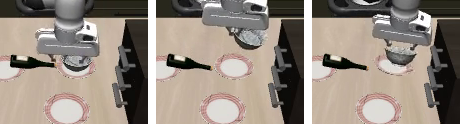
\includegraphics[width=.86\linewidth]{../figures/t1-gap-bat.png}\par
{\small\makebox[.286\linewidth]{142 · Tiếp cận}%
\makebox[.286\linewidth]{240 · Giữ bát đã nhấc}%
\makebox[.286\linewidth]{409 · Đạt mốc}\par}
\caption{Cận cảnh robot gắp và nhấc bát trong lượt T1}
\label{fig:t1-grasp-detail}
\end{figure}

\subsection{Hiệu chuẩn sau khi cho phép sai khác nguồn bộ ghi}
\label{sec:d2-calibration}

% claim-id: d2-calibration-override
Kiểm tra truy vấn theo sự kiện được dự kiến lặp lại trên nhóm trạng thái seen thứ hai, gồm states 12--19 của T1 và T3. Lần preflight nghiêm ngặt dừng trước khi có rollout, vì 7/14 mã băm nguồn của bộ ghi sự kiện khác với bản kê lưu cùng adapter. Để có số liệu chẩn đoán, hai arm được chạy lại với cờ \texttt{writer\_override=true}, ghi rõ trong manifest. Hai arm dùng cùng checkpoint F1, seed 42 và bảng mã băm nguồn, nhưng được khởi chạy từ hai Git revision khác nhau. Cả hai hoàn tất 16/16 episode, và hash trạng thái khởi tạo khớp ở cả 16 cặp. Kết quả trong mục này vì vậy là chẩn đoán phát triển theo đúng cấu hình đã chạy, không thay thế cohort calibration nghiêm ngặt.

\begin{table}[htbp]
\centering\small
\caption{Kết quả kiểm tra truy vấn theo sự kiện trên nhóm hiệu chuẩn sau override trên states 12--19 (16 episode mỗi arm)}
\label{tab:d2-calibration-results}
\setlength{\tabcolsep}{4pt}
\begin{tabular}{lrrrrr}
\toprule
\textbf{Arm} & \textbf{Thành công} & \shortstack{\textbf{SCR}\\\textbf{trung bình}} & \textbf{Overshoot} & \shortstack{\textbf{Lần gọi VLA}\\\textbf{/lượt}} & \shortstack{\textbf{Lượt có}\\\textbf{gọi sớm}} \\
\midrule
Shadow-projected & 1/16 & 0,188 & 2/16 & 95,50 & 0/16 \\
Event-projected & 1/16 & 0,083 & 0/16 & 101,69 & 16/16 \\
\bottomrule
\end{tabular}
\end{table}

Bảng~\ref{tab:d2-calibration-results} cho thấy hai arm có cùng tỷ lệ thành công 1/16, và cả hai lượt thành công đều thuộc T1. Event thành công ở state 18, nơi shadow thất bại; ngược lại, shadow thành công ở state 19, nơi event thất bại. Hai trường hợp bất đồng này có chiều ngược nhau, nên cohort không cho thấy chênh lệch về thành công giữa hai chế độ. Nhánh event phát tổng cộng 33 lần gọi sớm. Mỗi episode có một lần gọi sớm ở bước 3, khi fact đầu tiên của bộ nhớ xuất hiện, và 13/16 episode có thêm từ một đến hai lần gọi muộn hơn. Lượt thành công ở state 18 có ba lần gọi sớm, tại các bước 3, 285 và 399; mức này không khác các lượt thất bại trong cùng arm. Do đó, không thể quy thành công của lượt này cho việc truy vấn sớm.

Khác biệt đáng chú ý nhất nằm ở overshoot. Ở T1 states 12 và 13, shadow hoàn thành mốc yêu cầu nhưng tiếp tục chu kỳ và bị bộ chấm dừng sớm, nên SCR trung bình của shadow cao hơn dù không thêm lượt thành công. Event không có overshoot ở cả 16 lượt. Với chỉ hai lượt, quan sát này chỉ phù hợp với giả thuyết của RQ2 rằng truy vấn theo bằng chứng có thể hạn chế hành vi vượt mốc; nó chưa đủ để kết luận. Trên T3, cả hai arm đều 0/8.

\section{Can thiệp bỏ bộ nhớ tại một truy vấn}
\label{sec:e45-one-query}

% claim-id: e4-e5-one-query-ablation
Các phép đối sánh vòng kín ở trên đo kết quả cuối lượt nhưng không cho biết một dữ kiện bộ nhớ cụ thể có tác động đến quỹ đạo hay không. Để khảo sát tầng quyết định cục bộ của RQ1, khóa luận thực hiện can thiệp phản thực tế tại đúng một truy vấn của hai lượt kiểm tra truy vấn theo sự kiện thành công: T1 state 7 ở arm event, tại truy vấn bước 142, và T1 state 5 ở arm shadow, tại truy vấn bước 10. Mỗi ca có hai nhánh chạy từ cùng trạng thái, seed, checkpoint F1, bộ ghi và bộ điều phối. Nhánh \emph{F1-original} lặp lại đúng lời nhắc của lượt gốc. Nhánh \emph{F1-off-one-query} chỉ bỏ phần văn bản bộ nhớ tại truy vấn được chọn; mọi truy vấn khác giữ nguyên cơ chế sinh lời nhắc. Trước điểm can thiệp, cả hai nhánh phải khớp ảnh RGB và mọi đoạn hành động với lượt gốc.

\begin{table}[htbp]
\centering\small
\caption{Can thiệp bỏ bộ nhớ tại một truy vấn trên hai lượt kiểm tra truy vấn theo sự kiện thành công. ``Hết bước'' nghĩa là lượt dừng ở giới hạn 1.000 bước mà chưa đạt mốc}
\label{tab:e45-one-query}
\setlength{\tabcolsep}{3.5pt}
\begin{tabular}{llrrrrl}
\toprule
\textbf{Ca} & \textbf{Nhánh} & \shortstack{\textbf{Hành động}\\\textbf{trùng gốc}} & \shortstack{\textbf{$L_2$ hành}\\\textbf{động đầu}} & \shortstack{\textbf{$L_2$}\\\textbf{cả đoạn}} & \textbf{SCR} & \textbf{Kết quả} \\
\midrule
State 7, q142 & F1-original & 1.000/1.000 & 0 & 0 & 1 & Thành công \\
 & F1-off-one-query & 142/1.000 & 0,188 & 0,529 & 0 & Hết bước \\
\midrule
State 5, q10 & F1-original & 1.000/1.000 & 0 & 0 & 1 & Thành công \\
 & F1-off-one-query & 10/1.000 & 0,150 & 0,618 & 0 & Hết bước \\
\bottomrule
\end{tabular}
\end{table}

Bảng~\ref{tab:e45-one-query} cho thấy hai nhánh đối chứng tái lập chính xác 1.000/1.000 hành động của lượt gốc và đều thành công. Kết quả này xác nhận rằng môi trường và chính sách là tất định trong cấu hình đã dùng, nên mọi khác biệt sau điểm can thiệp đều xuất phát từ thay đổi lời nhắc. Ở cả hai ca, việc bỏ bộ nhớ tại một truy vấn giữ nguyên phần tiền tố 142/142 và 10/10 hành động, sau đó làm đoạn hành động đầu tiên lệch với khoảng cách $L_2$ lần lượt 0,188 và 0,150. Từ điểm này, không còn hành động nào trùng lượt gốc, và cả hai nhánh kết thúc ở giới hạn 1.000 bước mà không đạt mốc nào. Nội dung bị bỏ là fact ``bowl: 0 observed returns.'', ở ca state 7 có kèm nhãn ``History incomplete''.

Kết quả trên là bằng chứng về độ nhạy cục bộ của rollout đối với lời nhắc tại một truy vấn, quan sát ở hai ca cụ thể. Có ba giới hạn cần nêu rõ. Thứ nhất, hai ca được chọn có chủ đích từ các lượt thành công hiếm hoi của kiểm tra truy vấn theo sự kiện, nên không đại diện cho phân phối rollout. Thứ hai, thiết kế chưa có nhánh đối chứng giả, tức là thay lời nhắc bằng một biến thể có cùng mức khác biệt về văn bản nhưng không bỏ fact bộ nhớ. Vì thế chưa thể tách tác động của nội dung bộ nhớ khỏi tác động chung của việc thay đổi lời nhắc lên một quỹ đạo vốn nhạy với nhiễu. Thứ ba, fact bị bỏ mang thông tin tiến độ ban đầu, chưa phải fact xác nhận một chu kỳ đã hoàn thành. Hai ca này bổ sung cho phép thăm dò tám nhánh tại T1 state 16 nêu ở Chương 2, trong đó thay đổi dữ kiện tiến độ làm đoạn hành động lệch với $L_2$ từ 2,715 đến 4,306. Điểm mới của can thiệp bỏ bộ nhớ tại một truy vấn là có đối chứng tái lập chính xác và có kết quả cuối lượt. Chúng chưa ước lượng hiệu quả của bộ nhớ.

\section{Duy trì kỹ năng cơ sở trên LIBERO-10}
\label{sec:e6-retention}

Phép đánh giá này đo mức duy trì hiệu năng sau tinh chỉnh trên các tác vụ LIBERO-10 gốc bằng cách đối sánh với B0, checkpoint nền trước khi tinh chỉnh trong khóa luận. Trên mỗi mô hình nền, các điều kiện được chạy trên 10 tác vụ LIBERO-10 với 5 trạng thái khởi tạo mỗi tác vụ, cùng trạng thái và seed giữa các điều kiện. F1-off dùng trọng số F1 nhưng chỉ nhận chỉ dẫn gốc, vì các tác vụ LIBERO-10 không có lời nhắc bộ nhớ. Hai mô hình nền dùng ID trạng thái, nhịp điều khiển và runtime khác nhau, nên các chênh lệch giữa hai mô hình chỉ mang tính mô tả.

\subsection{SmolVLA}

% claim-id: e6-retention
Trên SmolVLA, thực nghiệm đánh giá khả năng duy trì kỹ năng thao tác cơ sở sau khi tinh chỉnh thông qua việc đối đầu giữa B0 gốc và F1-off trên 10 tác vụ của bộ benchmark LIBERO-10, với 5 trạng thái khởi tạo cho mỗi tác vụ (tổng cộng 50 cặp đối sánh). Cả hai điều kiện đều chạy trên cùng trạng thái và cùng seed ngẫu nhiên.

\begin{table}[htbp]
\centering\small
\caption{Tỷ lệ thành công sau tinh chỉnh trên 10 tác vụ LIBERO-10}
\label{tab:e6-retention-results}
\begin{tabular}{l*{10}{c}r}
\toprule
\textbf{Mô hình} & \textbf{0} & \textbf{1} & \textbf{2} & \textbf{3} & \textbf{4} & \textbf{5} & \textbf{6} & \textbf{7} & \textbf{8} & \textbf{9} & \textbf{Tổng} \\
\midrule
B0     & 0 & 3 & 5 & 5 & 3 & 5 & 4 & 4 & 3 & 5 & 37/50 (74\%) \\
F1-off & 2 & 1 & 2 & 5 & 2 & 0 & 2 & 3 & 3 & 3 & 23/50 (46\%) \\
\bottomrule
\end{tabular}
\end{table}

Bảng~\ref{tab:e6-retention-results} ghi nhận 37/50 thành công ở B0 và 23/50 ở F1-off; trong 50 cặp, có 19 lượt chỉ B0 thành công, 5 lượt chỉ F1-off thành công, 18 lượt cả hai thành công và 8 lượt cả hai thất bại. Khoảng bootstrap ghép cặp 95\% cho chênh lệch F1-off trừ B0 là $[-42;-14]$ điểm phần trăm, có điều kiện trên roster LIBERO-10 local này. Đánh giá duy trì hiệu năng sau tinh chỉnh mô tả khác biệt giữa hai cấu hình, không xác định nguyên nhân và không cô lập tác động nhân quả của memory.

Hình~\ref{fig:e6-retention-by-task} cho thấy mức duy trì khác nhau giữa các tác vụ. Chẳng hạn, ở tác vụ 3 (đặt bát vào ngăn dưới rồi đóng ngăn kéo), cả hai cấu hình đạt 5/5. Ở tác vụ 5 (đặt sách vào ngăn sau của hộp đựng), B0 đạt 5/5 còn F1-off đạt 0/5.

\begin{figure}[htbp]
\centering
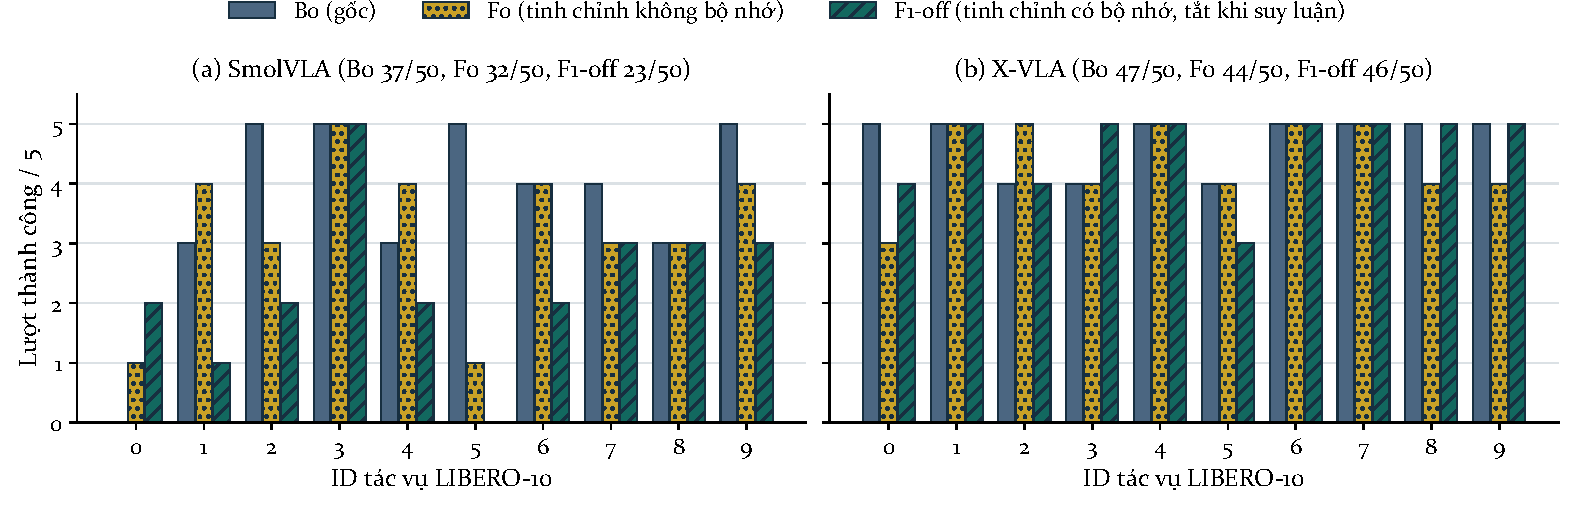
\includegraphics[width=.96\linewidth]{../figures/duy-tri-e6.pdf}
\caption{Số lượt thành công theo tác vụ của SmolVLA trên LIBERO-10}
\label{fig:e6-retention-by-task}
\end{figure}

Ở trạng thái 17 của tác vụ 5, nhật ký ghi B0 đạt vị từ đích. F1-off nhấc và đưa sách tới hộp nhưng kết thúc ở giới hạn 1.000 bước khi vị từ đích vẫn chưa đạt. Hình~\ref{fig:e6-book-placement} minh họa lượt F1-off, cùng trạng thái khởi tạo và seed 3559 với lượt B0.

\begin{figure}[htbp]
\centering
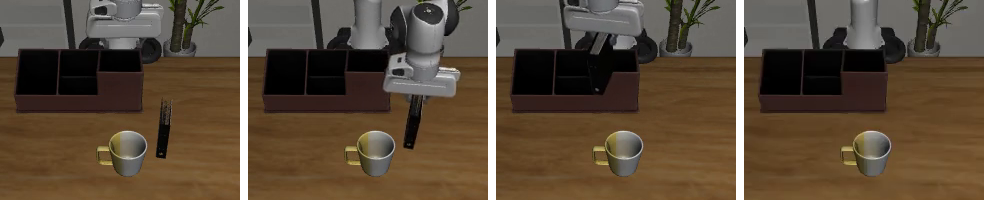
\includegraphics[width=.96\linewidth]{../figures/e6-dat-sach.png}\par
{\small\makebox[.24\linewidth]{Khung 0}%
\makebox[.24\linewidth]{Khung 77}%
\makebox[.24\linewidth]{Khung 103}%
\makebox[.24\linewidth]{Khung 1.000}\par}
\caption{F1-off nhấc sách nhưng chưa đặt đúng ngăn trong LIBERO-10}
\label{fig:e6-book-placement}
\end{figure}

\subsection{X-VLA}

% claim-id: xvla-e6-retention
Trên X-VLA, đánh giá duy trì hiệu năng sau tinh chỉnh gồm ba điều kiện B0, F0 và F1-off, với 50 bộ ba và 150 episode. Cấu hình X-VLA được mô tả ở Mục~\ref{sec:xvla-setup}. Các lượt chạy dùng client LIBERO của nhóm tác giả X-VLA, 10 bước ổn định ban đầu, tối đa 900 bước chính sách mỗi lượt, và seed mỗi episode được xác định từ ID tác vụ và ID trạng thái. Task, state và seed trùng nhau ở cả 50 bộ ba.

\begin{table}[htbp]
\centering\small
\caption{Số lượt thành công của X-VLA trong phép đánh giá duy trì hiệu năng sau tinh chỉnh theo tác vụ LIBERO-10 (mỗi ô trên 5 lượt)}
\label{tab:xvla-e6-results}
\begin{tabular}{l*{10}{c}r}
\toprule
\textbf{Điều kiện} & \textbf{0} & \textbf{1} & \textbf{2} & \textbf{3} & \textbf{4} & \textbf{5} & \textbf{6} & \textbf{7} & \textbf{8} & \textbf{9} & \textbf{Tổng} \\
\midrule
B0     & 5 & 5 & 4 & 4 & 5 & 4 & 5 & 5 & 5 & 5 & 47/50 (94\%) \\
F0     & 3 & 5 & 5 & 4 & 5 & 4 & 5 & 5 & 4 & 4 & 44/50 (88\%) \\
F1-off & 4 & 5 & 4 & 5 & 5 & 3 & 5 & 5 & 5 & 5 & 46/50 (92\%) \\
\bottomrule
\end{tabular}
\end{table}

\begin{table}[htbp]
\centering\small
\caption{Đối sánh ghép cặp giữa các điều kiện X-VLA trong phép đánh giá duy trì hiệu năng sau tinh chỉnh (50 cặp)}
\label{tab:xvla-e6-paired}
\setlength{\tabcolsep}{4pt}
\begin{tabular}{lrrrrrr}
\toprule
\textbf{So sánh A với B} & \shortstack{\textbf{Chỉ A}\\\textbf{đúng}} & \shortstack{\textbf{Chỉ B}\\\textbf{đúng}} & \shortstack{\textbf{Cả hai}\\\textbf{đúng}} & \shortstack{\textbf{Cả hai}\\\textbf{sai}} & \shortstack{\textbf{B trừ A}\\\textbf{(điểm \%)}} & \shortstack{\textbf{Bootstrap 95\%}\\\textbf{(điểm \%)}} \\
\midrule
B0 với F0     & 4 & 1 & 43 & 2 & $-6$ & $[-14;\,2]$ \\
B0 với F1-off & 3 & 2 & 44 & 1 & $-2$ & $[-10;\,6]$ \\
F0 với F1-off & 3 & 5 & 41 & 1 & $+4$ & $[-6;\,16]$ \\
\bottomrule
\end{tabular}
\end{table}

Bảng~\ref{tab:xvla-e6-results} và Bảng~\ref{tab:xvla-e6-paired} cho thấy cả hai adapter X-VLA giữ tỷ lệ thành công gần mức của B0 trên roster này. So với B0, F0 giảm 6 điểm phần trăm và F1-off giảm 2 điểm phần trăm. Số cặp bất đồng nhỏ, từ 5 đến 8 cặp mỗi so sánh, và mọi khoảng bootstrap ghép cặp 95\% đều chứa 0; kiểm định McNemar chính xác cho $p = 0{,}375$ với B0 so với F0 và $p = 1$ với B0 so với F1-off. Vì B0 đã đạt 94\%, cohort gần mức trần và chỉ phát hiện được mức suy giảm lớn. Kết quả vì vậy cho phép nói rằng trên roster này không quan sát thấy suy giảm lớn, nhưng không đủ để khẳng định tương đương. Chiều rộng khoảng tin cậy, khoảng 16 điểm phần trăm, cho thấy một mức suy giảm đến 10 điểm phần trăm vẫn phù hợp với dữ liệu.

Đặt cạnh kết quả SmolVLA, hai mô hình nền cho bức tranh khác nhau. Trên SmolVLA, F1-off thấp hơn B0 28 điểm phần trăm; trên X-VLA, mức chênh tương ứng là 2 điểm phần trăm. Do hai mô hình khác nhau về số tham số được cập nhật, biểu diễn hành động, độ dài đoạn hành động, roster trạng thái và runtime, khác biệt này chưa thể quy cho một nhân tố riêng lẻ. Mặt khác, đánh giá duy trì hiệu năng sau tinh chỉnh X-VLA chỉ đo khi bộ nhớ tắt, nên nó trả lời câu hỏi duy trì kỹ năng của RQ3 chứ không cho biết bộ nhớ có giúp X-VLA trên tác vụ phụ thuộc lịch sử hay không. Kết quả cũng mới dựa trên một seed cho mỗi trạng thái.

\section{Tổng hợp theo câu hỏi nghiên cứu}
\label{sec:ch4-rq-summary}

\textbf{RQ1, giá trị của bộ nhớ.} Đối sánh vòng kín không cho thấy lợi ích của bộ nhớ đối với tỷ lệ hoàn thành tác vụ: F1 đạt 0/40 so với 4/40 của F0, với khoảng bootstrap 95\% của chênh lệch nằm hoàn toàn dưới 0. Ở tầng quyết định cục bộ, can thiệp bỏ bộ nhớ tại một truy vấn cho thấy việc bỏ fact bộ nhớ tại một truy vấn đủ làm thay đổi đoạn hành động và kết cục của hai lượt thành công được chọn, trong khi đối chứng tái lập chính xác. Hai tầng này phù hợp với nhau: chính sách có phản ứng với lời nhắc bộ nhớ, nhưng phản ứng đó chưa chuyển hóa thành cải thiện tỷ lệ thành công trong cấu hình hiện tại. Bằng chứng hiện có chưa phân định được tác động riêng của nội dung bộ nhớ so với tác động chung của thay đổi lời nhắc.

\textbf{RQ2, độ tin cậy và lịch sử không đầy đủ.} Phép kiểm tra truy vấn theo sự kiện xác nhận rằng kiến trúc của đóng góp thứ hai vận hành trong vòng kín: truy vấn sớm được phát khi bộ nhớ đổi ngữ nghĩa và có mã evidence, còn nhãn ``History incomplete'' xuất hiện khi lịch sử chưa đủ. Ở cohort development, shadow và event đều đạt 1/24 thành công. Cohort calibration sau \texttt{writer\_override=true} cũng đạt 1/16 mỗi arm; do preflight nghiêm ngặt bị chặn vì 7/14 hash nguồn writer không khớp bản kê của adapter, đây chỉ là kết quả chẩn đoán. Trong cohort đó có 2/16 lượt overshoot ở shadow và 0/16 ở event. Quy mô và nguồn chạy này chỉ đủ để nêu giả thuyết cho các lượt xác nhận sau.

\textbf{RQ3, duy trì kỹ năng và mở rộng kiến trúc.} Hai mô hình nền cho mức chênh lệch sau tinh chỉnh khác nhau trong các cấu hình được đánh giá. Trên SmolVLA, F1-off thấp hơn B0 28 điểm phần trăm với khoảng tin cậy không chứa 0. Trên X-VLA, cả F0 và F1-off đều giữ tỷ lệ gần B0, và không quan sát thấy suy giảm lớn trên roster 50 trạng thái. Công thức thích ứng F0/F1 đã được áp dụng cho một kiến trúc thứ hai có biểu diễn hành động tuyệt đối. Tuy nhiên, khả năng mở rộng của chính cơ chế bộ nhớ sang X-VLA chưa được đo, vì các lượt X-VLA trên LIBERO-Mem chưa đủ cohort.

Tổng thể, các kết quả hỗ trợ đóng góp thứ hai ở mức vận hành của kiến trúc và hỗ trợ đóng góp thứ ba ở mức một quy trình đánh giá tách bạch giữa tầng quyết định cục bộ, tầng vòng kín và tầng duy trì kỹ năng. Kết quả chưa xác lập lợi ích tổng quát của bộ nhớ đối với tỷ lệ hoàn thành tác vụ. Chương 5 thảo luận các giới hạn này và các thực nghiệm cần bổ sung.
